% The Model Context Protocol: wrap a resource once, not once per client.
% ---------------------------------------------------------------------------
% style.tex --- shared preamble for every figure in book/figures/tikz/
%
% One style for all figures: Latin Modern, thin black lines, a light grey
% fill, and one accent colour used only to mark what is untrusted or wrong.
% Build with scripts/build_figures.sh; see book/figures/README.md.
% ---------------------------------------------------------------------------
\documentclass[tikz,border=6pt]{standalone}
\usepackage[T1]{fontenc}
\usepackage{lmodern}
\usetikzlibrary{arrows.meta,positioning,shapes.geometric,calc,fit,backgrounds}

\hyphenpenalty=10000   % short lines in boxes: ragged, never hyphenated

\definecolor{lightgrey}{gray}{0.92}
\definecolor{accent}{HTML}{9B2D20}

\tikzset{
  every picture/.style={
    line width=0.6pt,
    font=\small,
    >={Stealth[length=5pt,width=4pt]},
    node distance=14pt and 24pt,
  },
  % shapes
  box/.style={draw, rectangle, inner xsep=8pt, inner ysep=5pt,
              minimum height=22pt, align=center},
  grey/.style={box, fill=lightgrey},
  rounded/.style={box, rounded corners=9pt},
  decision/.style={draw, diamond, aspect=2.4, inner sep=1.5pt, align=center},
  group/.style={draw, dashed, rounded corners=5pt, inner sep=7pt},
  % text
  tag/.style={font=\footnotesize, align=center, inner sep=2pt},
  note/.style={font=\footnotesize\itshape, align=center, inner sep=2pt},
  code/.style={font=\small\ttfamily},
  codetag/.style={font=\footnotesize\ttfamily, align=center, inner sep=2pt},
  title/.style={font=\small\scshape, align=center, inner sep=2pt},
  % lines
  arrow/.style={->},
  back/.style={->, dashed},
  thin/.style={line width=0.4pt, gray},
  % the one accent, for what is untrusted, wrong or missing
  bad/.style={accent},
  badbox/.style={box, draw=accent, text=accent},
}

\begin{document}
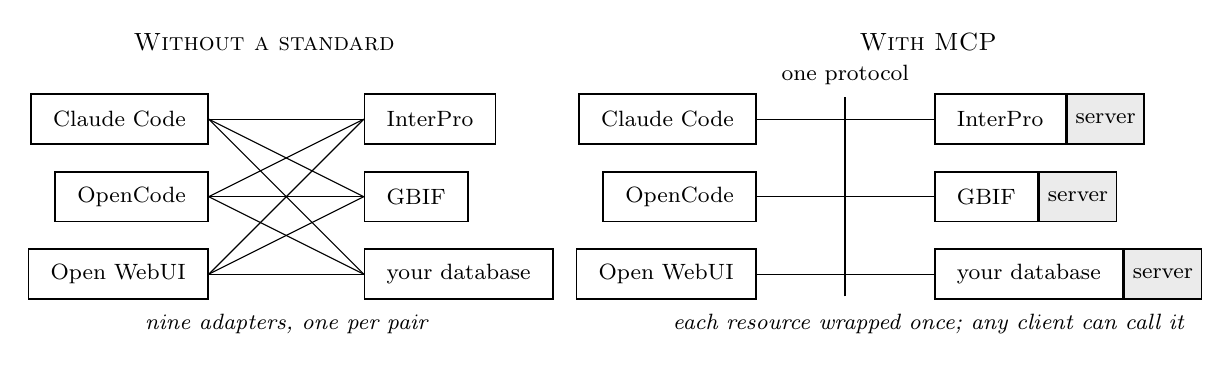
\begin{tikzpicture}[small/.style={box, minimum height=18pt, inner ysep=3pt, font=\footnotesize}]
  % Left: one adapter per pair
  \node[title] at (60pt,56pt) {Without a standard};
  \foreach \i/\n in {1/Claude Code,2/OpenCode,3/Open WebUI}
    \node[small, anchor=east] (c\i) at (40pt,{(2-\i)*28pt}) {\n};
  \foreach \i/\n in {1/InterPro,2/GBIF,3/your database}
    \node[small, anchor=west] (r\i) at (96pt,{(2-\i)*28pt}) {\n};
  \foreach \i in {1,2,3} \foreach \j in {1,2,3} \draw[thin, black] (c\i.east) -- (r\j.west);
  \node[note] at (68pt,-46pt) {nine adapters, one per pair};
  % Right: one wrapper per resource
  \node[title] at (300pt,56pt) {With MCP};
  \foreach \i/\n in {1/Claude Code,2/OpenCode,3/Open WebUI}
    \node[small, anchor=east] (d\i) at (238pt,{(2-\i)*28pt}) {\n};
  \foreach \i/\n in {1/InterPro,2/GBIF,3/your database}
    \node[small, anchor=west] (s\i) at (302pt,{(2-\i)*28pt}) {\n};
  \foreach \i in {1,2,3} \node[small, fill=lightgrey, anchor=west, minimum width=0pt, inner xsep=3pt]
    (w\i) at (s\i.east) {server};
  \draw (270pt,-36pt) -- (270pt,36pt);
  \foreach \i in {1,2,3} \draw[thin, black] (d\i.east) -- (270pt,{(2-\i)*28pt});
  \foreach \i in {1,2,3} \draw[thin, black] (270pt,{(2-\i)*28pt}) -- (s\i.west);
  \node[tag] at (270pt,44pt) {one protocol};
  \node[note] at (300pt,-46pt) {each resource wrapped once; any client can call it};
\end{tikzpicture}
\end{document}
